\documentclass{article}
\usepackage{amsmath}
\usepackage{amssymb}
\usepackage{graphicx}
\usepackage{hyperref}
\usepackage[version=4]{mhchem}

\title{Problem 5}
\date{}

\begin{document}
\maketitle

\section*{Problem}
Two circles intersect in \(A\) and \(B\), and the measure of the common chord \(A B=10\). The line joining the centers cuts the circles in \(P\) and \(Q\). If \(P Q=3\) and the measure of the radius of one circle is 13 , find the radius of the other circle. (Note that the illustration is not drawn to scale.)\\
\centering
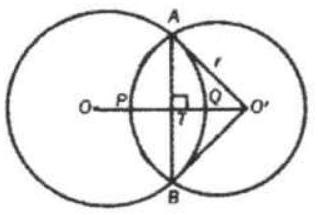
\includegraphics[width=\textwidth]{images/problem_image_1.jpg}

\section*{Solution}
\(\frac{41}{8}\).\\
Since \(O^{\prime} A=O^{\prime} B\) and \(O A=O B, O O^{\prime}\) is the perpendicular bisector of \(A B\).\\
Therefore, in right \(\triangle A T O\), since \(A O=13\) and \(A T=5\), we find \(O T=12\). Since \(O Q\) \(=13\) (also a radius of circle \(O\) ), and \(O T=12, T Q=1\). We Know that \(P Q=3\). \(P T\) \(=P Q-T Q\); therefore, \(P T=2\). Let \(O^{\prime} A=O^{\prime} P=r\), and \(P T=2, T O^{\prime}=r-2\).\\
Applying the Pythagorean Theorem in tight \(\triangle A T O^{\prime},(A T)^{2}+(T O)^{2}=(A O)^{2}\).\\
Substituting, \(5^{2}+(r-2)^{2}=r^{2}\), and \(r=\frac{29}{4}\). \(P T=P Q+T Q\); therefore, \(P T=4\).\\
Again, let \(O^{\prime} A=O^{\prime} P=r\) then \(T O^{\prime}=r-4\).\\
Applying the Pythagorean Theorem in right \(\triangle A T O^{\prime}\),\\
\((A T)^{2}+(T O)^{2}=(A O)^{2}\).\\
Substituting, \(5^{2}+(r-4)^{2}=r^{2}\), and \(r=\frac{41}{8}\).\\
\centering
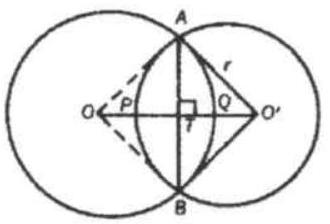
\includegraphics[width=\textwidth]{images/reasoning_image_1.jpg}

\end{document}
